\section{Macro Benchmarks}
In order to not skew results towards \ac{JIT} compilers, because microbenchmarks are likely to be misleading \cite{sestoft2013microbenchmarks, microbenchmarkmislead}, we also implement a macro benchmark.
Some sources claim that \ac{JIT} provies speedup on loops, although according to a recent study this is not always the case \cite{vmwarmup}.
\todo{ref to that one source that says micro benchmarks favour \ac{JIT} due to loops - please tell me we have one}

\input{sections/04-benchmarking/hot-and-cold.tex}

\subsection{Test Cases}
In order to establish a manageable size of macro benchmark, we brainstormed and evaluated a series of test cases. The ideas are as follows:
\begin{description}
    \item[Angry Physics] This test case is reminiscent of the game Angry Birds, hence the name. In this test a series of 3D objects (boxes, balls, pyramids, etc.) is placed on a platform. A canon that shoots is place at a distance from the platform. This canon will shoot projectiles of different size, mass and shape at the platform to trigger collisions and gravity simulation.
    \item[Wumpus World] In this case a 2D grid-based board is placed in the world. In the world an agent must collect a treasure and return to the start. The world is also inhabited by wumpuses, that wish to eat the agent. There are also a series of pits which the agent must avoid. The agent can sense wumpuses and pits on neighbouring grids by stenches and breezes respectively \cite{wumpus:world}.
    \item[Cowichan Problems] The Cowichan problems is a series of thirteen problems that mainly revolves around matrix and vector calculations \cite{wilson1995assessing}. The sizes of the matrices and vectors can be scaled to fit the size of the test and the problems chained to test different aspects of a language.
    \item[Game of Life] Game of Life is a cellular automaton described by John Conway \cite{game:of:life}. In the game organisms can be placed in a grid world. There are a series of rules, that determines how the organisms will evolve or die, that needs to be evaluated for each organism.
\end{description}

% Wumpus world: http://aima.cs.berkeley.edu/slides-pdf/chapter07-6pp.pdf
% Lund Universitet Applied Artificial Intelligence: http://cs.lth.se/edaf70/course-material/
Though not a traditional macro benchmark, we chose to implement the Wumpus World. The reasons for this choice is that it is somewhat reminiscent of a game, being that it has an \ac{AI}-element along with the possibility of adding graphics. Even though it is a simulation of an \ac{AI} it has a deterministic behaviour on a given map.

\subsection{Rules in Wumpus World}
The Wumpus World is an N x M grid world. Each cell may contain one object. The Wumpus World uses the term \textit{neighbouring cells}. Given a cell X, it's neighbouring cells are that to the north, east, south or west of X. The cells on the diagonal is thus not considered as neighbours. A visual representation, as presented in \cite{wumpus:world}, is shown in \figureref{wumpus:world}.
A Wumpus can give off a stench so the agent know where the Wumpus could be, the same goes for for pits that have breezes next to it. 
Last there is Glitter which is the treasure, the agent wins when it gets back to start position (0,0), with the treasure.

\begin{figure}
    \centering
    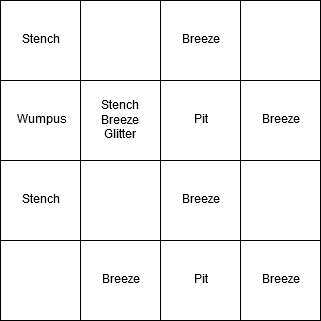
\includegraphics[width=.5\textwidth]{images/wumpus.png}
    \caption{A 4 x 4 Wumpus World with one Wumpus and two pits \cite{wumpus:world}}
    \label{fig:wumpus:world}
\end{figure}
\todo{Vi kan tilføje nogle farver til figuren. Vil det gøre det lettere?}

An agent may take one of a couple of actions in each turn. They are as follows:
\begin{description}
    \item[Forward] The agent moves one step forward in its current direction.
    \item[Turn] The agent turns either left or right to change its direction.
    \item[Grab] The agent picks up the content of the current cell.
    \item[Release] The agent releases what ever it is holding and places it on the current grid cell.
    \item[Shoot] The agent shoots an arrow forwards from its current position to kill a wumpus in front of it.
    \item[Climb] The agent may climb out of the cave if it's located in the start position.
\end{description}

The agent is \dquote{blind} and may only perceive the world through percepts. The percepts are tied to objects, which are as follows:
\begin{description}
    \item[Agent] The agent is an \ac{AI}. It has a starting position and a goal of retrieving a treasure in the world. It must do so while minimising the score, i.e. the number of actions it has taken.
    \item[Wumpus] Wumpuses are hostile towards the agent. If the agent ends up in the same cell as a Wumpus, it will die. Wumpuses give of stench to the neighbouring cells. If the agent is sure of the location of a Wumpus, it may shoot to kill it (in which case the agent perceives a scream).
    \item[Pit] A pit is a hole in the ground. The agent will die if it falls into a pit and pits give of a breeze to neighbouring cells.
    \item[Treasure] There is one treasure in each map. The agent has the goal of getting to the treasure, picking it up and going back to the start state. A treasure gives off glitter to the cell it is placed in.
\end{description}
Apart from said percepts, the agent will perceive a bump if it walks into a wall.

\subsection{Simplifications}
In the implementation we make a couple of simplifications from the description in \cite{wumpus:world}. The first is that we abstract away the bump perception and instead assume that the agent knows its current position in the world.
The agent also knows where it has been, so it remembers its path.

Regarding the agent's actions several changes were made. We did so because the actions presented in \cite{wumpus:world} seemed a bit terse, most likely because they are meant to represent an actual robot. As a precise robot simulation is not desired in this case, we argue that the simplifications won't do any harm\todo{Meh. We should probably write something more scientific here.}. The actions were changed as follows:
\begin{description}
    \item[Grab and Release] The grab and release actions are replaced with a boolean flag to indicate whether or not the agent has reached the cell that holds the gold. If the agent is in the start cell with the flag set to true, the map is completed.
    \item[Turn and Forward] The turn and forward actions are replace with a \ttt{Move(direction)}-action, that moves the agent in the given direction. Direction either being north, west, east or south.
    \item[Climb] Finally the Climb action was removed and instead a map is completed when the agent reaches back to the start cell or dies from walking into a pit or a wumpus.
\end{description}

\subsection{Platforms}
We chose Unity and Unreal for the test. Unity was chosen because it, according to statista.com in 2014, was used by 62\% of the responses in their survey \cite{gameengine:statista}.
Unreal was chosen because it was the fastest of all the engines in the micro benchmarks (see \secref{micro-benchmarking}).

In this experiment we do not include a functional language, as we were not able to find a decent game engine with a functional language.

\subsection{Metrics}
Unlike the micro benchmarks that had a predefined metric of measuring time, macro benchmarks does not. In order to formulate a baseline for the discussion on which metric to use, a series of questions were formulated:
\begin{itemize}
    \item How many worlds can we spawn at once while still producing at least 60 \ac{FPS}?
    \item How many \ac{FPS} can we get from iterating each tick?
    \item How much time does one update take?
    \item What is the memory footprint per Wumpus World?
\end{itemize}
The first two questions are tied to the fact, that the macrobenchmarks are run in a game engine. In the context of games it makes sense, as it is the metrics most often used by gamers. However, they make very little sense if the macrobenchmarks are not intended to test a game engine.

The third question has the advantage, that it pairs well with the metrics used in the microbenchmarks and the fourth, that memory is also a performance concern, that we have not discussed previously in this project.

We choose to examine the last two questions by reusing the timer code that was written for the microbenchmarks along with examining memory use per instance of the wumpus world.

\subsection{Results}
\begin{figure}
    \centering
    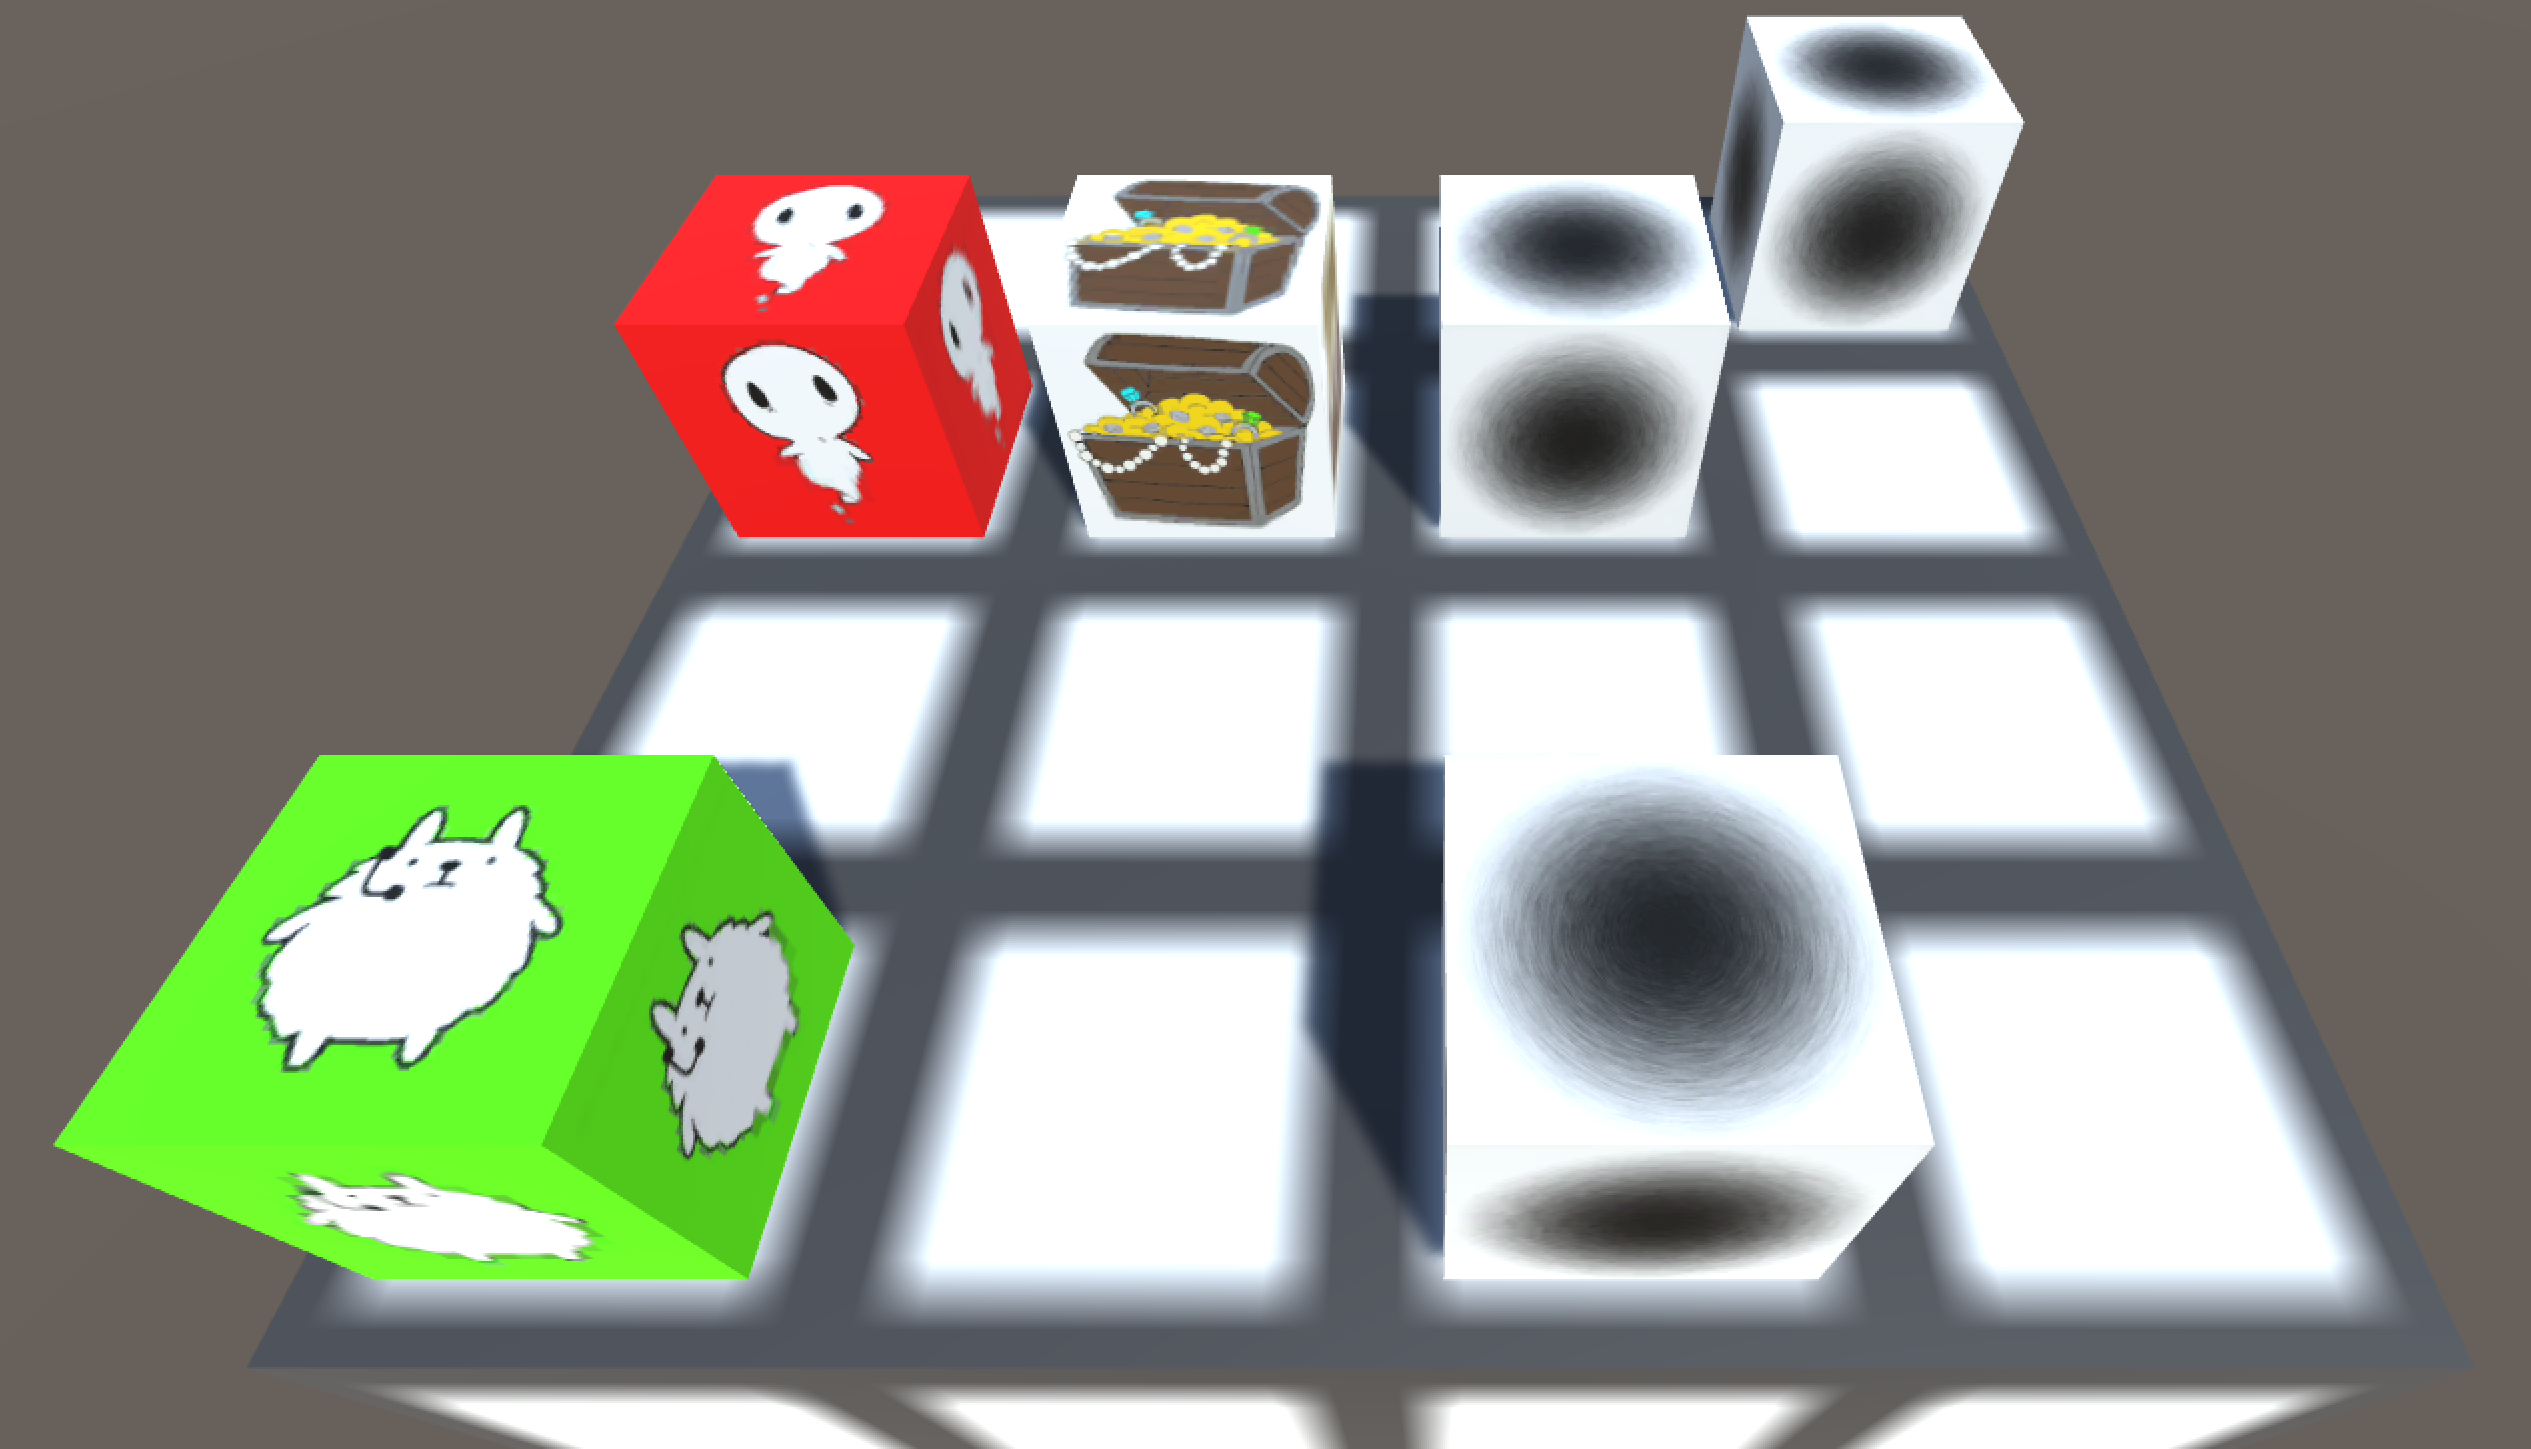
\includegraphics[width=\textwidth]{images/Wumpus_Unity.png}
    \caption{Wumpus implementation in Unity, the map is the same as in \figureref{wumpus:world}}
    \label{fig:wumpus:world:unity}
\end{figure}

\begin{figure}[H]
    \makebox[\textwidth][c]{
    \begin{tikzpicture}
    \tikzset{every mark/.append style={scale=.5}}
        \begin{axis}[
                width=1.25\textwidth, 
                height= 8cm,
                ymin = 0,
                ymax = 2,
                xmin = 0,
                xmax = 130,
            ]
            \addplot[mark=*, color=red] table [x={Iteration No.}, y=Unreal] {\macroData};
            \addplot[mark=*, color=blue] table [x={Iteration No.}, y=Unity] {\macroData};
        \end{axis}
    \end{tikzpicture}}
    \caption{Macrobenchmark Results}
    \label{fig:macro-results}
\end{figure}